\documentclass[a4paper,11pt,twocolumn]{article}

\usepackage{icphs2023}
\usepackage{metalogo} % Only needed for the XeLaTeX logo
\usepackage{epstopdf}

\hyphenpenalty=10000 % no hyphenation

\title{Paper template for {ICPhS} 2023 Prague}
\author{Please write XXX instead of the name(s) of the author(s)}
\organization{Please write XXX instead of the affiliation(s)}
\email{please write XXX instead of the email address(es)}
\begin{document}

\maketitle

\begin{abstract}
This is the layout specification and template definition for the papers of ICPhS XX (the 20th International Congress of Phonetic Sciences, which will be held in Prague, Czech Republic, August 7-11, 2023). This template is a revised version of the one used for Melbourne ICPhS XIX in 2019, originally generated from the template for Speech Prosody 2006 in Dresden.

The abstract may consist of more than one paragraph but must be kept within a 150-word limit. This abstract will be printed in the abstract booklet to be given out at the conference.
\end{abstract}

\keywords{There is space for up to five self-selected keywords
  (maximum two lines).}


\section{Introduction}

The following rules apply to all submitted papers:

\begin{itemize}
\item they must be written in English
\item they must not contain the name(s) of the author(s) (for
anonymous review)
\item the maximum is four pages for Congress papers, plus up to one additional page of references. Papers for Plenary lectures can be longer
\item they must be submitted in PDF format (cf.\ Section~4)
\item the paper submission will occur via a web interface
\end{itemize}
This paper template can be found on the conference website. If there
are special questions or wishes regarding paper preparation and
submission for ICPhS 2023, correspondence should be addressed to
icphs2023@guarant.cz. Information for full paper submission will be
available on the web at \url{https://www.icphs2023.org/}.



\section{Page layout and style}

The page layout should conform to the following rules. By far the easiest way to meet these requirements is to use the supplied templates and check details against this example file. If for some reason you cannot use the template, please follow these rules as carefully as possible, or contact the editors at icphs2023@guarant.cz for further instructions.

\subsection{Basic layout features}

\begin{itemize}
\item The layout is appropriate for A4 format.
\item Two columns are used
  except for the title part and possibly for large figures that need a
  full page width.
\item Left margin is 20 mm. Right margin will depend on
  the size of the paper. Column width is 80 mm.
\item Spacing between
  columns is 10 mm.
\item Top margin 25 mm (except first page which has 30
  mm to the title top). Bottom margin will depend on the size of the
  paper.
\item Text height (without headers and footers) is a maximum of
  235 mm.  Headers and footers should be left empty
\item Check indentations
  and spacings by comparing with this example file.
\end{itemize}

\subsubsection{Headings}

Section headings are centered in boldface with capitalized letters. Sub-headings start at the left margin in the column with the first letter capitalized and the rest of the heading in lower case. Sub-sub-headings appear like sub-headings, except that they are in italics and not boldface. See examples in this file. No more than 3 levels of headings should be used.  Empty lines should be left above and below each section heading.

\subsection{Text font}

Times or Times New Roman font is used for the main text. Recommended font size is 11 points. Other font types may be used if needed for special purposes. If using any non-Unicode fonts, these must be embedded in the final PDF file.

The \LaTeX{} template can be used either with plain \LaTeX{} or \XeLaTeX.

\subsection{Figures}

All figures should be centered on the column (or page, if the figure
spans both columns). Figure captions should follow each figure and
have the format given in Fig.~\ref{fig:vowels}.

Figures should preferably be line drawings. If they contain grey
shades or colours, it should be checked that they print well on a
high-quality noncolour laser printer.

\begin{figure}[!ht]
\begin{center}
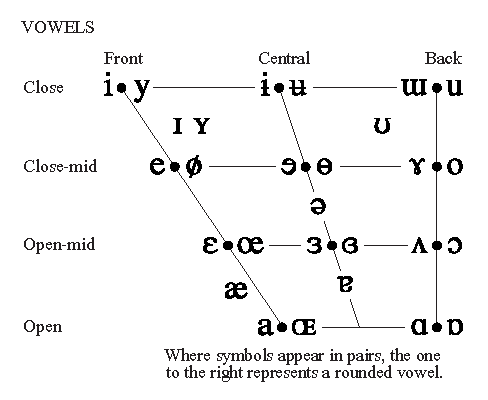
\includegraphics[width=6cm]{ipa.eps}
\caption{The vowel chart used in the International Phonetic
Alphabet (IPA).}\label{fig:vowels}
\end{center}
\end{figure}

\subsection{Tables}

An example of a table is shown as Table~\ref{tab:decibel}.  Somewhat
different styles are allowed according to the type and purpose of the
table. Colour should not be used, but grey shading is allowed. There
should be a margin of 6~points (pt) above and below the table.

The caption text may be above or below the table, but this should be
consistent throughout the submission. Left and right indentation of
the caption should be 0.5~cm.

\begin{table}[!ht]
\begin{center}
\begin{tabular}{|c|c|}
\hline
\rowcolor[gray]{.75}
ratio    & Decibels\\
\hline
$1/1$    & $0$\\
$2/1$    & $6$\\
$3.16$   & $10$\\
$1/10$   & $-20$\\
$10/1$   & $20$\\
$100/1$  & $40$\\
$1000/1$ & $60$\\
\hline
\end{tabular}
\caption{This is an example of a table showing Decibel (dB)
ratios.}\label{tab:decibel}
\end{center}
\end{table}


\subsection{Equations}

Equations should be placed on separate lines and numbered. An example
of an equation is
\begin{equation}\label{eq:tzero}
T_0 = \frac{1}{f_0}.
\end{equation}
Numbers of equations can be on the right or on the left margin of the
text column.

\subsection{Examples}

Examples from other languages can either be presented in the body text, or, if referred to elsewhere or particularly long and complex, can be put on a separate, numbered line, as should be done for equations.


\subsection{Phonetic fonts}

We recommend that you use the \textsc{tipa} package for IPA phonetic symbols. For information about how to access Unicode fonts in the Word template, see \cite{IPA-SIL} or \cite{IPA-KEYBOARD}. The font you use must be embedded. Please remember to check this,  e.g. by inspecting the ``Document Properties --- Fonts'' in Acrobat Reader.


\subsection{Page numbering}

Page numbers will be added electronically to the document
later. \textit{Please do not add page numbers and please do not insert
any footers or headers!}

\subsection{References}

Please use just the reference number in square brackets. Formulations
with author names like ``\ldots\ as Ladefoged~\cite{Ladefoged:2003}
showed that \ldots'' are acceptable but not ``as shown in [Ladefoged,
3]'' or ``as shown in (Ladefoged~[3])''.

References are to be numbered in chronological order. Please
double-check the final version of your paper with regard to the
correct correspondence of references to their numbers.

\subsection{Hyperlinks}

Links to URLs or email addresses should be formatted as normal text,
\textit{not} as hyperlinks and not blue or underlined etc. Usually
hyperlinks to web pages are listed in the references section. If
required, line breaks can be placed within URLs after slashes or
dashes (cf.~\cite{IPA-SIL,IPA-KEYBOARD}), but doublecheck that no hyphens
are inserted.

\subsection{Footnotes and endnotes}

If footnotes cannot be avoided they should appear as
endnotes.\footnote{This footnote appears here as an endnote.}

\section{Multimedia files}

Multimedia data that are part of the paper are to be embedded in the submitted PDF; they cannot be submitted as supplementary data. Any images are to be included in the paper as Figures (see Section 2.3 above). It is the authors' responsibility to check image quality ahead of submission. Audio examples are to be embedded within the PDF. To do this, authors can generate the PDF, and then embed the audio files using Adobe Acrobat Professional, or other software that offers the same outcome, so that the audio is included in the PDF. The presence of audio data should be identified in the text.

We encourage authors to illustrate video data using still photographs from the video, and to include them as figures in the PDF.  We cannot accept embedded video files, but authors are welcome to refer readers to a URL on the internet where these can be viewed.


\section{PDF details}

PDF files submitted must comply with the following requirements:

\begin{enumerate}
\item all special fonts and symbols must be embedded in the PDF
  file so that correct rendering of the PDF does not depend on the
  fonts installed on the viewer's computer
\item there must be no
  password protection on the PDF file, i.e. PDF files must not be
  protected by PDF security in any way, i.e. content extraction,
  document assembly, high resolution printing etc. must not be
  forbidden
\item PDF files should not contain any colours, hyperlinks,
  multimedia or 3D content, and no JavaScript or forms
\item PDF files
  should be no larger than 5 MB.
\end{enumerate}
\section{Anonymity}

In ICPhS 2023 submissions, an anonymous reviewing process will be used. This means that for the first submission the name(s) of the author(s) and
their affiliation(s) \emph{must not} be mentioned. In addition, please refrain from using acknowledgements.  Please also try to make your own previous research as anonymous as possible. As an example: do not write ``In our previous study \cite{Stevens:1999} we could show\ldots'' but ``As shown in \cite{Stevens:1999}\ldots''. Or refer to your own published or otherwise widely known work, and to that of the other authors, in the ``Julius Caesar style'', i.e. in the third person (for example: his work, her work, their work). Reference as ``anonymous'' only work that you or the other authors have submitted for publication, but which has not yet been published, e.g. \cite{Anonymous:submitted}.

Please make sure that no author details appear in the Document Properties of the PDF file. \emph{For the revised paper submission author details are of course needed}. Acknowledgements and references to one's own work are possible as usual.

\section{Format of references}

References are formatted using the IEEE standard (available in various reference management systems like Zotero or Mendeley). If you do not use a reference management system, please use the examples provided for monographs \cite{Fant:1960}, contributions to volumes \cite{Stevens:1999}, journal articles \cite{Beattie/etal:1982}, articles in conference proceedings \cite{Ladefoged:2003}. Abbreviations of
well-known conferences and journals are possible \cite{Peterson/Barney:1952}. Software tools \cite{Boril/Skarnitzl:2016} are referenced according to authors' instructions. 

\bibliographystyle{IEEEtran}
\bibliography{icphs2023}

\theendnotes

\end{document}
